% Options for packages loaded elsewhere
\PassOptionsToPackage{unicode}{hyperref}
\PassOptionsToPackage{hyphens}{url}
%
\documentclass[
]{article}
\usepackage{amsmath,amssymb}
\usepackage{lmodern}
\usepackage{iftex}
\ifPDFTeX
  \usepackage[T1]{fontenc}
  \usepackage[utf8]{inputenc}
  \usepackage{textcomp} % provide euro and other symbols
\else % if luatex or xetex
  \usepackage{unicode-math}
  \defaultfontfeatures{Scale=MatchLowercase}
  \defaultfontfeatures[\rmfamily]{Ligatures=TeX,Scale=1}
\fi
% Use upquote if available, for straight quotes in verbatim environments
\IfFileExists{upquote.sty}{\usepackage{upquote}}{}
\IfFileExists{microtype.sty}{% use microtype if available
  \usepackage[]{microtype}
  \UseMicrotypeSet[protrusion]{basicmath} % disable protrusion for tt fonts
}{}
\makeatletter
\@ifundefined{KOMAClassName}{% if non-KOMA class
  \IfFileExists{parskip.sty}{%
    \usepackage{parskip}
  }{% else
    \setlength{\parindent}{0pt}
    \setlength{\parskip}{6pt plus 2pt minus 1pt}}
}{% if KOMA class
  \KOMAoptions{parskip=half}}
\makeatother
\usepackage{xcolor}
\IfFileExists{xurl.sty}{\usepackage{xurl}}{} % add URL line breaks if available
\IfFileExists{bookmark.sty}{\usepackage{bookmark}}{\usepackage{hyperref}}
\hypersetup{
  pdfauthor={Mestrado em Bioestatística (UEM); Aluno João Matheus Slujala Krüger Taborda Hneda; Profª. Dra. Isolde Terezinha Santos Previdelli},
  hidelinks,
  pdfcreator={LaTeX via pandoc}}
\urlstyle{same} % disable monospaced font for URLs
\usepackage[left=1.1cm,right=1.1cm,top=1.75cm,bottom=1.75cm]{geometry}
\usepackage{color}
\usepackage{fancyvrb}
\newcommand{\VerbBar}{|}
\newcommand{\VERB}{\Verb[commandchars=\\\{\}]}
\DefineVerbatimEnvironment{Highlighting}{Verbatim}{commandchars=\\\{\}}
% Add ',fontsize=\small' for more characters per line
\usepackage{framed}
\definecolor{shadecolor}{RGB}{248,248,248}
\newenvironment{Shaded}{\begin{snugshade}}{\end{snugshade}}
\newcommand{\AlertTok}[1]{\textcolor[rgb]{0.94,0.16,0.16}{#1}}
\newcommand{\AnnotationTok}[1]{\textcolor[rgb]{0.56,0.35,0.01}{\textbf{\textit{#1}}}}
\newcommand{\AttributeTok}[1]{\textcolor[rgb]{0.77,0.63,0.00}{#1}}
\newcommand{\BaseNTok}[1]{\textcolor[rgb]{0.00,0.00,0.81}{#1}}
\newcommand{\BuiltInTok}[1]{#1}
\newcommand{\CharTok}[1]{\textcolor[rgb]{0.31,0.60,0.02}{#1}}
\newcommand{\CommentTok}[1]{\textcolor[rgb]{0.56,0.35,0.01}{\textit{#1}}}
\newcommand{\CommentVarTok}[1]{\textcolor[rgb]{0.56,0.35,0.01}{\textbf{\textit{#1}}}}
\newcommand{\ConstantTok}[1]{\textcolor[rgb]{0.00,0.00,0.00}{#1}}
\newcommand{\ControlFlowTok}[1]{\textcolor[rgb]{0.13,0.29,0.53}{\textbf{#1}}}
\newcommand{\DataTypeTok}[1]{\textcolor[rgb]{0.13,0.29,0.53}{#1}}
\newcommand{\DecValTok}[1]{\textcolor[rgb]{0.00,0.00,0.81}{#1}}
\newcommand{\DocumentationTok}[1]{\textcolor[rgb]{0.56,0.35,0.01}{\textbf{\textit{#1}}}}
\newcommand{\ErrorTok}[1]{\textcolor[rgb]{0.64,0.00,0.00}{\textbf{#1}}}
\newcommand{\ExtensionTok}[1]{#1}
\newcommand{\FloatTok}[1]{\textcolor[rgb]{0.00,0.00,0.81}{#1}}
\newcommand{\FunctionTok}[1]{\textcolor[rgb]{0.00,0.00,0.00}{#1}}
\newcommand{\ImportTok}[1]{#1}
\newcommand{\InformationTok}[1]{\textcolor[rgb]{0.56,0.35,0.01}{\textbf{\textit{#1}}}}
\newcommand{\KeywordTok}[1]{\textcolor[rgb]{0.13,0.29,0.53}{\textbf{#1}}}
\newcommand{\NormalTok}[1]{#1}
\newcommand{\OperatorTok}[1]{\textcolor[rgb]{0.81,0.36,0.00}{\textbf{#1}}}
\newcommand{\OtherTok}[1]{\textcolor[rgb]{0.56,0.35,0.01}{#1}}
\newcommand{\PreprocessorTok}[1]{\textcolor[rgb]{0.56,0.35,0.01}{\textit{#1}}}
\newcommand{\RegionMarkerTok}[1]{#1}
\newcommand{\SpecialCharTok}[1]{\textcolor[rgb]{0.00,0.00,0.00}{#1}}
\newcommand{\SpecialStringTok}[1]{\textcolor[rgb]{0.31,0.60,0.02}{#1}}
\newcommand{\StringTok}[1]{\textcolor[rgb]{0.31,0.60,0.02}{#1}}
\newcommand{\VariableTok}[1]{\textcolor[rgb]{0.00,0.00,0.00}{#1}}
\newcommand{\VerbatimStringTok}[1]{\textcolor[rgb]{0.31,0.60,0.02}{#1}}
\newcommand{\WarningTok}[1]{\textcolor[rgb]{0.56,0.35,0.01}{\textbf{\textit{#1}}}}
\usepackage{graphicx}
\makeatletter
\def\maxwidth{\ifdim\Gin@nat@width>\linewidth\linewidth\else\Gin@nat@width\fi}
\def\maxheight{\ifdim\Gin@nat@height>\textheight\textheight\else\Gin@nat@height\fi}
\makeatother
% Scale images if necessary, so that they will not overflow the page
% margins by default, and it is still possible to overwrite the defaults
% using explicit options in \includegraphics[width, height, ...]{}
\setkeys{Gin}{width=\maxwidth,height=\maxheight,keepaspectratio}
% Set default figure placement to htbp
\makeatletter
\def\fps@figure{htbp}
\makeatother
\setlength{\emergencystretch}{3em} % prevent overfull lines
\providecommand{\tightlist}{%
  \setlength{\itemsep}{0pt}\setlength{\parskip}{0pt}}
\setcounter{secnumdepth}{-\maxdimen} % remove section numbering
\usepackage{fancyhdr}
\ifLuaTeX
  \usepackage{selnolig}  % disable illegal ligatures
\fi

\title{Lista de Exercícios II - Bioestatística (DES4060 - Turma 2022)}
\author{Mestrado em Bioestatística (UEM) \and Aluno João Matheus Slujala
Krüger Taborda Hneda \and Profª. Dra. Isolde Terezinha Santos
Previdelli}
\date{}

\begin{document}
\maketitle

\renewcommand*\contentsname{Sumário}
{
\setcounter{tocdepth}{5}
\tableofcontents
}
\newpage

\hypertarget{especificauxe7uxf5es}{%
\section{Especificações}\label{especificauxe7uxf5es}}

Encontrar alguma distribuição de probabilidade nova (pelo menos 2
parâmetros) e:

\begin{itemize}
\tightlist
\item
  escrever quem fez, onde usou, como usou, propriedades
\item
  implementar as funções d, p, q r
\item
  fazer figuras
\item
  realizar estudo de simulação (estimação máxima verossimilhança) --
  variar tamanho da amostra e ver como as estimativas mudam, viés, rmse
\end{itemize}

\hypertarget{escrever-quem-fez-onde-usou-como-usou-propriedades}{%
\section{Escrever quem fez, onde usou, como usou,
propriedades}\label{escrever-quem-fez-onde-usou-como-usou-propriedades}}

\hypertarget{implementar-as-funuxe7uxf5es-d-p-q-r}{%
\section{Implementar as funções d, p, q,
r}\label{implementar-as-funuxe7uxf5es-d-p-q-r}}

\begin{Shaded}
\begin{Highlighting}[]
\CommentTok{\# f(x)}
\NormalTok{dKwMOE }\OtherTok{\textless{}{-}} \ControlFlowTok{function}\NormalTok{(x,a, b, p, lambda)}
\NormalTok{\{}
\NormalTok{    dexp }\OtherTok{\textless{}{-}} \FunctionTok{dexp}\NormalTok{(}\AttributeTok{x=}\NormalTok{x,}\AttributeTok{rate=}\NormalTok{lambda)}
\NormalTok{    pexp }\OtherTok{\textless{}{-}} \FunctionTok{pexp}\NormalTok{(}\AttributeTok{q=}\NormalTok{x,}\AttributeTok{rate=}\NormalTok{lambda)}
    
\NormalTok{    dKwMOE\_p1 }\OtherTok{\textless{}{-}}\NormalTok{ (a}\SpecialCharTok{*}\NormalTok{b}\SpecialCharTok{*}\NormalTok{(}\DecValTok{1}\SpecialCharTok{{-}}\NormalTok{p)}\SpecialCharTok{*}\NormalTok{dexp}\SpecialCharTok{*}\NormalTok{(pexp}\SpecialCharTok{\^{}}\NormalTok{(a}\DecValTok{{-}1}\NormalTok{))) }\SpecialCharTok{/}\NormalTok{ ((}\DecValTok{1}\SpecialCharTok{{-}}\NormalTok{p}\SpecialCharTok{*}\NormalTok{(}\DecValTok{1}\SpecialCharTok{{-}}\NormalTok{pexp))}\SpecialCharTok{\^{}}\NormalTok{(a}\SpecialCharTok{+}\DecValTok{1}\NormalTok{))}
\NormalTok{    dKwMOE\_p2 }\OtherTok{\textless{}{-}}\NormalTok{ (}\DecValTok{1} \SpecialCharTok{{-}}\NormalTok{ ((pexp)}\SpecialCharTok{/}\NormalTok{(}\DecValTok{1} \SpecialCharTok{{-}}\NormalTok{ p}\SpecialCharTok{*}\NormalTok{(}\DecValTok{1}\SpecialCharTok{{-}}\NormalTok{pexp)))}\SpecialCharTok{\^{}}\NormalTok{a )}\SpecialCharTok{\^{}}\NormalTok{(b}\DecValTok{{-}1}\NormalTok{)}
\NormalTok{    dKwMOE\_p1 }\SpecialCharTok{*}\NormalTok{ dKwMOE\_p2}
\NormalTok{\}}


\NormalTok{dKwMOE\_curve }\OtherTok{\textless{}{-}} \ControlFlowTok{function}\NormalTok{(a, b, p, lambda,}
                         \AttributeTok{col=}\StringTok{"blue"}\NormalTok{,}\AttributeTok{lwd=}\DecValTok{2}\NormalTok{,}\AttributeTok{xlab=}\StringTok{"x"}\NormalTok{,}\AttributeTok{ylab=}\StringTok{"f(x)"}\NormalTok{,}\AttributeTok{xlim =} \FunctionTok{c}\NormalTok{(}\DecValTok{0}\NormalTok{, }\FloatTok{1.8}\NormalTok{), }\AttributeTok{ylim =} \FunctionTok{c}\NormalTok{(}\DecValTok{0}\NormalTok{, }\DecValTok{10}\NormalTok{),}\AttributeTok{add=}\ConstantTok{FALSE}\NormalTok{) \{}
    \FunctionTok{curve}\NormalTok{(}
        \FunctionTok{dKwMOE}\NormalTok{(}
\NormalTok{            x,}
            \AttributeTok{a =}\NormalTok{ a,}
            \AttributeTok{b =}\NormalTok{ b,}
            \AttributeTok{p =}\NormalTok{ p,}
            \AttributeTok{lambda =}\NormalTok{ lambda}
\NormalTok{        ),}
        \AttributeTok{col =}\NormalTok{ col, }\CommentTok{\# cor}
        \CommentTok{\#lty=1, \# tipo}
        \AttributeTok{lwd =}\NormalTok{ lwd, }\CommentTok{\# tamanho}
        \AttributeTok{xlab =}\NormalTok{ xlab,}
        \AttributeTok{ylab =}\NormalTok{ ylab,}
        \AttributeTok{xlim =}\NormalTok{ xlim,}
        \AttributeTok{ylim =}\NormalTok{ ylim,}
        \AttributeTok{add =}\NormalTok{ add}
\NormalTok{    )}
    
\NormalTok{\}}


\NormalTok{params }\OtherTok{\textless{}{-}} \FunctionTok{list}\NormalTok{(}\AttributeTok{a=}\FunctionTok{c}\NormalTok{(}\FloatTok{12.0}\NormalTok{,}\FloatTok{10.0}\NormalTok{,}\FloatTok{0.5}\NormalTok{,}\FloatTok{15.0}\NormalTok{),}
               \AttributeTok{b=}\FunctionTok{c}\NormalTok{(}\FloatTok{5.0}\NormalTok{,}\FloatTok{2.0}\NormalTok{,}\FloatTok{2.5}\NormalTok{,}\FloatTok{10.0}\NormalTok{),}
               \AttributeTok{p=}\FunctionTok{c}\NormalTok{(}\FloatTok{0.5}\NormalTok{,}\FloatTok{0.5}\NormalTok{,}\FloatTok{0.2}\NormalTok{,}\FloatTok{0.1}\NormalTok{),}
               \AttributeTok{lambda=}\FunctionTok{c}\NormalTok{(}\FloatTok{2.5}\NormalTok{,}\FloatTok{2.5}\NormalTok{,}\FloatTok{2.5}\NormalTok{,}\FloatTok{2.5}\NormalTok{),}
               \AttributeTok{col=}\FunctionTok{c}\NormalTok{(}\StringTok{"blue"}\NormalTok{,}\StringTok{"red"}\NormalTok{,}\StringTok{"black"}\NormalTok{,}\StringTok{"gray"}\NormalTok{))}

\FunctionTok{dKwMOE\_curve}\NormalTok{(}\AttributeTok{a =}\NormalTok{ params}\SpecialCharTok{$}\NormalTok{a[}\DecValTok{1}\NormalTok{],  }\AttributeTok{b =}\NormalTok{ params}\SpecialCharTok{$}\NormalTok{b[}\DecValTok{1}\NormalTok{], }\AttributeTok{p =}\NormalTok{ params}\SpecialCharTok{$}\NormalTok{p[}\DecValTok{1}\NormalTok{], }\AttributeTok{lambda =}\NormalTok{ params}\SpecialCharTok{$}\NormalTok{lambda[}\DecValTok{1}\NormalTok{], }\AttributeTok{col=}\NormalTok{params}\SpecialCharTok{$}\NormalTok{col[}\DecValTok{1}\NormalTok{], }\AttributeTok{add=}\ConstantTok{FALSE}\NormalTok{)}
\FunctionTok{dKwMOE\_curve}\NormalTok{(}\AttributeTok{a =}\NormalTok{ params}\SpecialCharTok{$}\NormalTok{a[}\DecValTok{2}\NormalTok{],  }\AttributeTok{b =}\NormalTok{ params}\SpecialCharTok{$}\NormalTok{b[}\DecValTok{2}\NormalTok{], }\AttributeTok{p =}\NormalTok{ params}\SpecialCharTok{$}\NormalTok{p[}\DecValTok{2}\NormalTok{], }\AttributeTok{lambda =}\NormalTok{ params}\SpecialCharTok{$}\NormalTok{lambda[}\DecValTok{2}\NormalTok{], }\AttributeTok{col=}\NormalTok{params}\SpecialCharTok{$}\NormalTok{col[}\DecValTok{2}\NormalTok{], }\AttributeTok{add=}\ConstantTok{TRUE}\NormalTok{)}
\FunctionTok{dKwMOE\_curve}\NormalTok{(}\AttributeTok{a =}\NormalTok{ params}\SpecialCharTok{$}\NormalTok{a[}\DecValTok{3}\NormalTok{],  }\AttributeTok{b =}\NormalTok{ params}\SpecialCharTok{$}\NormalTok{b[}\DecValTok{3}\NormalTok{], }\AttributeTok{p =}\NormalTok{ params}\SpecialCharTok{$}\NormalTok{p[}\DecValTok{3}\NormalTok{], }\AttributeTok{lambda =}\NormalTok{ params}\SpecialCharTok{$}\NormalTok{lambda[}\DecValTok{3}\NormalTok{], }\AttributeTok{col=}\NormalTok{params}\SpecialCharTok{$}\NormalTok{col[}\DecValTok{3}\NormalTok{], }\AttributeTok{add=}\ConstantTok{TRUE}\NormalTok{)}
\FunctionTok{dKwMOE\_curve}\NormalTok{(}\AttributeTok{a =}\NormalTok{ params}\SpecialCharTok{$}\NormalTok{a[}\DecValTok{4}\NormalTok{],  }\AttributeTok{b =}\NormalTok{ params}\SpecialCharTok{$}\NormalTok{b[}\DecValTok{4}\NormalTok{], }\AttributeTok{p =}\NormalTok{ params}\SpecialCharTok{$}\NormalTok{p[}\DecValTok{4}\NormalTok{], }\AttributeTok{lambda =}\NormalTok{ params}\SpecialCharTok{$}\NormalTok{lambda[}\DecValTok{4}\NormalTok{], }\AttributeTok{col=}\NormalTok{params}\SpecialCharTok{$}\NormalTok{col[}\DecValTok{4}\NormalTok{], }\AttributeTok{add=}\ConstantTok{TRUE}\NormalTok{)}
\FunctionTok{legend}\NormalTok{(}
    \StringTok{"topright"}\NormalTok{,}
    \AttributeTok{legend =} \FunctionTok{c}\NormalTok{(}
        \FunctionTok{paste0}\NormalTok{(}\StringTok{"a = "}\NormalTok{,params}\SpecialCharTok{$}\NormalTok{a[}\DecValTok{1}\NormalTok{],}\StringTok{",  b = "}\NormalTok{,params}\SpecialCharTok{$}\NormalTok{b[}\DecValTok{1}\NormalTok{],}\StringTok{"    p = "}\NormalTok{,params}\SpecialCharTok{$}\NormalTok{p[}\DecValTok{1}\NormalTok{],}\StringTok{", lambda = "}\NormalTok{,params}\SpecialCharTok{$}\NormalTok{lambda[}\DecValTok{1}\NormalTok{]),}
        \FunctionTok{paste0}\NormalTok{(}\StringTok{"a = "}\NormalTok{,params}\SpecialCharTok{$}\NormalTok{a[}\DecValTok{2}\NormalTok{],}\StringTok{",  b = "}\NormalTok{,params}\SpecialCharTok{$}\NormalTok{b[}\DecValTok{2}\NormalTok{],}\StringTok{"    p = "}\NormalTok{,params}\SpecialCharTok{$}\NormalTok{p[}\DecValTok{2}\NormalTok{],}\StringTok{", lambda = "}\NormalTok{,params}\SpecialCharTok{$}\NormalTok{lambda[}\DecValTok{2}\NormalTok{]),}
        \FunctionTok{paste0}\NormalTok{(}\StringTok{"a = "}\NormalTok{,params}\SpecialCharTok{$}\NormalTok{a[}\DecValTok{3}\NormalTok{],}\StringTok{",  b = "}\NormalTok{,params}\SpecialCharTok{$}\NormalTok{b[}\DecValTok{3}\NormalTok{],}\StringTok{"    p = "}\NormalTok{,params}\SpecialCharTok{$}\NormalTok{p[}\DecValTok{3}\NormalTok{],}\StringTok{", lambda = "}\NormalTok{,params}\SpecialCharTok{$}\NormalTok{lambda[}\DecValTok{3}\NormalTok{]),}
        \FunctionTok{paste0}\NormalTok{(}\StringTok{"a = "}\NormalTok{,params}\SpecialCharTok{$}\NormalTok{a[}\DecValTok{4}\NormalTok{],}\StringTok{",  b = "}\NormalTok{,params}\SpecialCharTok{$}\NormalTok{b[}\DecValTok{4}\NormalTok{],}\StringTok{"    p = "}\NormalTok{,params}\SpecialCharTok{$}\NormalTok{p[}\DecValTok{4}\NormalTok{],}\StringTok{", lambda = "}\NormalTok{,params}\SpecialCharTok{$}\NormalTok{lambda[}\DecValTok{4}\NormalTok{])}
\NormalTok{    ),}
    \AttributeTok{lty =} \DecValTok{1}\NormalTok{,}
    \AttributeTok{lwd =} \DecValTok{2}\NormalTok{,}
    \AttributeTok{col =}\NormalTok{ params}\SpecialCharTok{$}\NormalTok{col,}
\NormalTok{)}
\end{Highlighting}
\end{Shaded}

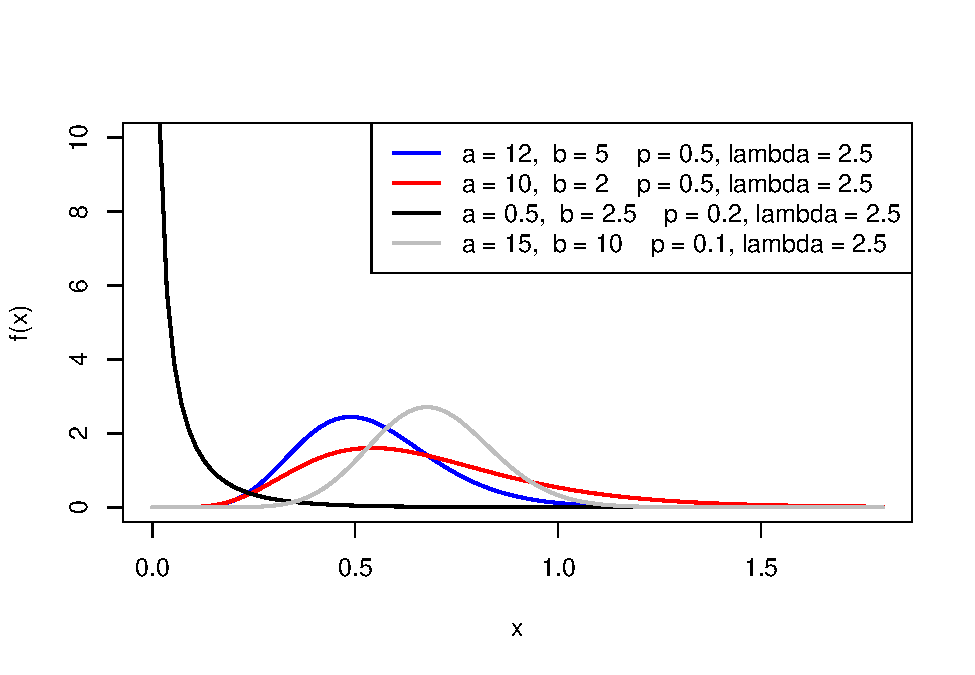
\includegraphics{Kumaraswamy_Marshall-Olkin_Exponential_distribution_files/figure-latex/dKwMOE com exp-1.pdf}

\begin{Shaded}
\begin{Highlighting}[]
\CommentTok{\# F(x)}
\NormalTok{pKwMOE }\OtherTok{\textless{}{-}} \ControlFlowTok{function}\NormalTok{(q, a, b, p, lambda)}
\NormalTok{\{}
\NormalTok{    pexp }\OtherTok{\textless{}{-}} \FunctionTok{pexp}\NormalTok{(}\AttributeTok{q=}\NormalTok{q,}\AttributeTok{rate=}\NormalTok{lambda)}
    
    \DecValTok{1} \SpecialCharTok{{-}}\NormalTok{ (}\DecValTok{1}\SpecialCharTok{{-}}\NormalTok{(pexp}\SpecialCharTok{/}\NormalTok{(}\DecValTok{1}\SpecialCharTok{{-}}\NormalTok{p}\SpecialCharTok{*}\NormalTok{(}\DecValTok{1}\SpecialCharTok{{-}}\NormalTok{pexp)))}\SpecialCharTok{\^{}}\NormalTok{a)}\SpecialCharTok{\^{}}\NormalTok{b}
\NormalTok{\}}


\NormalTok{pKwMOE\_curve }\OtherTok{\textless{}{-}} \ControlFlowTok{function}\NormalTok{(x,a, b, p, lambda,}
                         \AttributeTok{col=}\StringTok{"blue"}\NormalTok{,}\AttributeTok{lwd=}\DecValTok{2}\NormalTok{,}\AttributeTok{xlab=}\StringTok{"x"}\NormalTok{,}\AttributeTok{ylab=}\StringTok{"F(x)"}\NormalTok{,}\AttributeTok{xlim =} \FunctionTok{c}\NormalTok{(}\DecValTok{0}\NormalTok{, }\FloatTok{1.8}\NormalTok{), }\AttributeTok{ylim =} \FunctionTok{c}\NormalTok{(}\DecValTok{0}\NormalTok{, }\FloatTok{1.1}\NormalTok{),}\AttributeTok{add=}\ConstantTok{FALSE}\NormalTok{) \{}
    \FunctionTok{curve}\NormalTok{(}
        \FunctionTok{pKwMOE}\NormalTok{(}
            \AttributeTok{q =}\NormalTok{ x,}
            \AttributeTok{a =}\NormalTok{ a,}
            \AttributeTok{b =}\NormalTok{ b,}
            \AttributeTok{p =}\NormalTok{ p,}
            \AttributeTok{lambda =}\NormalTok{ lambda}
\NormalTok{        ),}
        \AttributeTok{col =}\NormalTok{ col, }\CommentTok{\# cor}
        \CommentTok{\#lty=1, \# tipo}
        \AttributeTok{lwd =}\NormalTok{ lwd, }\CommentTok{\# tamanho}
        \AttributeTok{xlab =}\NormalTok{ xlab,}
        \AttributeTok{ylab =}\NormalTok{ ylab,}
        \AttributeTok{xlim =}\NormalTok{ xlim,}
        \AttributeTok{ylim =}\NormalTok{ ylim,}
        \AttributeTok{add =}\NormalTok{ add}
\NormalTok{    )}
    
\NormalTok{\}}


\NormalTok{params }\OtherTok{\textless{}{-}} \FunctionTok{list}\NormalTok{(}\AttributeTok{a=}\FunctionTok{c}\NormalTok{(}\FloatTok{12.0}\NormalTok{,}\FloatTok{10.0}\NormalTok{,}\FloatTok{0.5}\NormalTok{,}\FloatTok{15.0}\NormalTok{),}
               \AttributeTok{b=}\FunctionTok{c}\NormalTok{(}\FloatTok{5.0}\NormalTok{,}\FloatTok{2.0}\NormalTok{,}\FloatTok{2.5}\NormalTok{,}\FloatTok{10.0}\NormalTok{),}
               \AttributeTok{p=}\FunctionTok{c}\NormalTok{(}\FloatTok{0.5}\NormalTok{,}\FloatTok{0.5}\NormalTok{,}\FloatTok{0.2}\NormalTok{,}\FloatTok{0.1}\NormalTok{),}
               \AttributeTok{lambda=}\FunctionTok{c}\NormalTok{(}\FloatTok{2.5}\NormalTok{,}\FloatTok{2.5}\NormalTok{,}\FloatTok{2.5}\NormalTok{,}\FloatTok{2.5}\NormalTok{),}
               \AttributeTok{col=}\FunctionTok{c}\NormalTok{(}\StringTok{"blue"}\NormalTok{,}\StringTok{"red"}\NormalTok{,}\StringTok{"black"}\NormalTok{,}\StringTok{"gray"}\NormalTok{))}

\FunctionTok{pKwMOE\_curve}\NormalTok{(}\AttributeTok{a =}\NormalTok{ params}\SpecialCharTok{$}\NormalTok{a[}\DecValTok{1}\NormalTok{],  }\AttributeTok{b =}\NormalTok{ params}\SpecialCharTok{$}\NormalTok{b[}\DecValTok{1}\NormalTok{], }\AttributeTok{p =}\NormalTok{ params}\SpecialCharTok{$}\NormalTok{p[}\DecValTok{1}\NormalTok{], }\AttributeTok{lambda =}\NormalTok{ params}\SpecialCharTok{$}\NormalTok{lambda[}\DecValTok{1}\NormalTok{], }\AttributeTok{col=}\NormalTok{params}\SpecialCharTok{$}\NormalTok{col[}\DecValTok{1}\NormalTok{], }\AttributeTok{add=}\ConstantTok{FALSE}\NormalTok{)}
\FunctionTok{pKwMOE\_curve}\NormalTok{(}\AttributeTok{a =}\NormalTok{ params}\SpecialCharTok{$}\NormalTok{a[}\DecValTok{2}\NormalTok{],  }\AttributeTok{b =}\NormalTok{ params}\SpecialCharTok{$}\NormalTok{b[}\DecValTok{2}\NormalTok{], }\AttributeTok{p =}\NormalTok{ params}\SpecialCharTok{$}\NormalTok{p[}\DecValTok{2}\NormalTok{], }\AttributeTok{lambda =}\NormalTok{ params}\SpecialCharTok{$}\NormalTok{lambda[}\DecValTok{2}\NormalTok{], }\AttributeTok{col=}\NormalTok{params}\SpecialCharTok{$}\NormalTok{col[}\DecValTok{2}\NormalTok{], }\AttributeTok{add=}\ConstantTok{TRUE}\NormalTok{)}
\FunctionTok{pKwMOE\_curve}\NormalTok{(}\AttributeTok{a =}\NormalTok{ params}\SpecialCharTok{$}\NormalTok{a[}\DecValTok{3}\NormalTok{],  }\AttributeTok{b =}\NormalTok{ params}\SpecialCharTok{$}\NormalTok{b[}\DecValTok{3}\NormalTok{], }\AttributeTok{p =}\NormalTok{ params}\SpecialCharTok{$}\NormalTok{p[}\DecValTok{3}\NormalTok{], }\AttributeTok{lambda =}\NormalTok{ params}\SpecialCharTok{$}\NormalTok{lambda[}\DecValTok{3}\NormalTok{], }\AttributeTok{col=}\NormalTok{params}\SpecialCharTok{$}\NormalTok{col[}\DecValTok{3}\NormalTok{], }\AttributeTok{add=}\ConstantTok{TRUE}\NormalTok{)}
\FunctionTok{pKwMOE\_curve}\NormalTok{(}\AttributeTok{a =}\NormalTok{ params}\SpecialCharTok{$}\NormalTok{a[}\DecValTok{4}\NormalTok{],  }\AttributeTok{b =}\NormalTok{ params}\SpecialCharTok{$}\NormalTok{b[}\DecValTok{4}\NormalTok{], }\AttributeTok{p =}\NormalTok{ params}\SpecialCharTok{$}\NormalTok{p[}\DecValTok{4}\NormalTok{], }\AttributeTok{lambda =}\NormalTok{ params}\SpecialCharTok{$}\NormalTok{lambda[}\DecValTok{4}\NormalTok{], }\AttributeTok{col=}\NormalTok{params}\SpecialCharTok{$}\NormalTok{col[}\DecValTok{4}\NormalTok{], }\AttributeTok{add=}\ConstantTok{TRUE}\NormalTok{)}
\FunctionTok{legend}\NormalTok{(}
    \StringTok{"bottomright"}\NormalTok{,}
    \AttributeTok{legend =} \FunctionTok{c}\NormalTok{(}
        \FunctionTok{paste0}\NormalTok{(}\StringTok{"a = "}\NormalTok{,params}\SpecialCharTok{$}\NormalTok{a[}\DecValTok{1}\NormalTok{],}\StringTok{",  b = "}\NormalTok{,params}\SpecialCharTok{$}\NormalTok{b[}\DecValTok{1}\NormalTok{],}\StringTok{"    p = "}\NormalTok{,params}\SpecialCharTok{$}\NormalTok{p[}\DecValTok{1}\NormalTok{],}\StringTok{", lambda = "}\NormalTok{,params}\SpecialCharTok{$}\NormalTok{lambda[}\DecValTok{1}\NormalTok{]),}
        \FunctionTok{paste0}\NormalTok{(}\StringTok{"a = "}\NormalTok{,params}\SpecialCharTok{$}\NormalTok{a[}\DecValTok{2}\NormalTok{],}\StringTok{",  b = "}\NormalTok{,params}\SpecialCharTok{$}\NormalTok{b[}\DecValTok{2}\NormalTok{],}\StringTok{"    p = "}\NormalTok{,params}\SpecialCharTok{$}\NormalTok{p[}\DecValTok{2}\NormalTok{],}\StringTok{", lambda = "}\NormalTok{,params}\SpecialCharTok{$}\NormalTok{lambda[}\DecValTok{2}\NormalTok{]),}
        \FunctionTok{paste0}\NormalTok{(}\StringTok{"a = "}\NormalTok{,params}\SpecialCharTok{$}\NormalTok{a[}\DecValTok{3}\NormalTok{],}\StringTok{",  b = "}\NormalTok{,params}\SpecialCharTok{$}\NormalTok{b[}\DecValTok{3}\NormalTok{],}\StringTok{"    p = "}\NormalTok{,params}\SpecialCharTok{$}\NormalTok{p[}\DecValTok{3}\NormalTok{],}\StringTok{", lambda = "}\NormalTok{,params}\SpecialCharTok{$}\NormalTok{lambda[}\DecValTok{3}\NormalTok{]),}
        \FunctionTok{paste0}\NormalTok{(}\StringTok{"a = "}\NormalTok{,params}\SpecialCharTok{$}\NormalTok{a[}\DecValTok{4}\NormalTok{],}\StringTok{",  b = "}\NormalTok{,params}\SpecialCharTok{$}\NormalTok{b[}\DecValTok{4}\NormalTok{],}\StringTok{"    p = "}\NormalTok{,params}\SpecialCharTok{$}\NormalTok{p[}\DecValTok{4}\NormalTok{],}\StringTok{", lambda = "}\NormalTok{,params}\SpecialCharTok{$}\NormalTok{lambda[}\DecValTok{4}\NormalTok{])}
\NormalTok{    ),}
    \AttributeTok{lty =} \DecValTok{1}\NormalTok{,}
    \AttributeTok{lwd =} \DecValTok{2}\NormalTok{,}
    \AttributeTok{col =}\NormalTok{ params}\SpecialCharTok{$}\NormalTok{col,}
\NormalTok{)}
\FunctionTok{abline}\NormalTok{(}\AttributeTok{h=}\DecValTok{1}\NormalTok{,}\AttributeTok{lty=}\DecValTok{2}\NormalTok{)}
\FunctionTok{abline}\NormalTok{(}\AttributeTok{h=}\FloatTok{0.5}\NormalTok{,}\AttributeTok{lty=}\DecValTok{2}\NormalTok{)}
\end{Highlighting}
\end{Shaded}

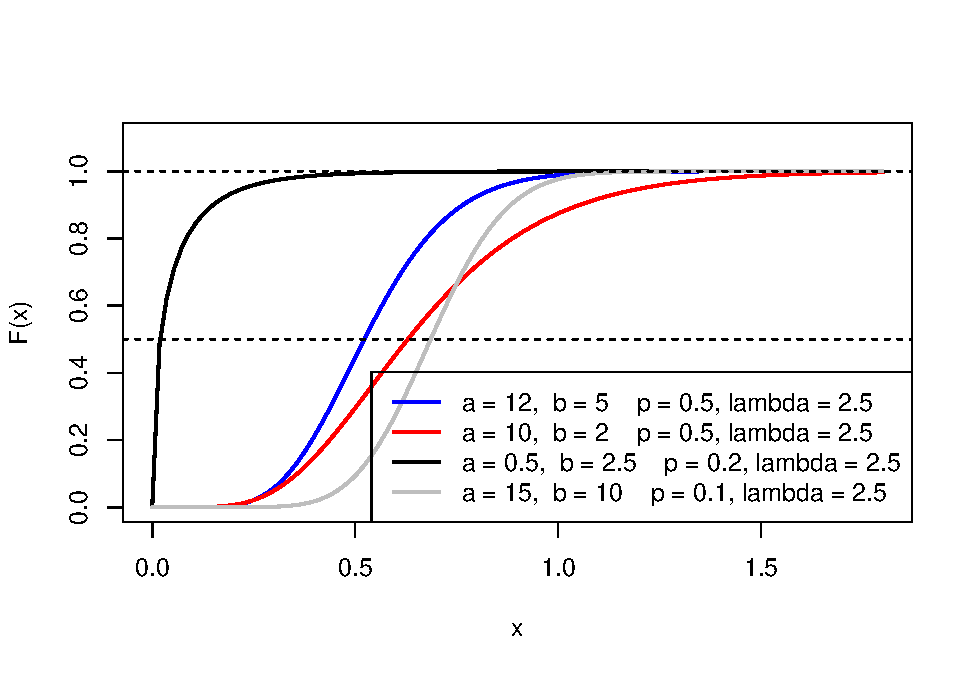
\includegraphics{Kumaraswamy_Marshall-Olkin_Exponential_distribution_files/figure-latex/pKwMOE com exp-1.pdf}

\begin{Shaded}
\begin{Highlighting}[]
\NormalTok{qKwMOE }\OtherTok{\textless{}{-}} \ControlFlowTok{function}\NormalTok{(}\AttributeTok{prob=}\FloatTok{0.5}\NormalTok{, a, b, p, lambda)}
\NormalTok{\{}
\NormalTok{    x\_q }\OtherTok{\textless{}{-}}\NormalTok{ (}\DecValTok{1}\SpecialCharTok{/}\NormalTok{lambda)}\SpecialCharTok{*}\FunctionTok{log}\NormalTok{( (}\DecValTok{1} \SpecialCharTok{{-}}\NormalTok{ p}\SpecialCharTok{*}\NormalTok{(}\DecValTok{1}\SpecialCharTok{{-}}\NormalTok{(}\DecValTok{1}\SpecialCharTok{{-}}\NormalTok{prob)}\SpecialCharTok{\^{}}\NormalTok{(}\DecValTok{1}\SpecialCharTok{/}\NormalTok{b))}\SpecialCharTok{\^{}}\NormalTok{(}\DecValTok{1}\SpecialCharTok{/}\NormalTok{a) ) }\SpecialCharTok{/}\NormalTok{ (}\DecValTok{1} \SpecialCharTok{{-}}\NormalTok{ (}\DecValTok{1}\SpecialCharTok{{-}}\NormalTok{(}\DecValTok{1}\SpecialCharTok{{-}}\NormalTok{prob)}\SpecialCharTok{\^{}}\NormalTok{(}\DecValTok{1}\SpecialCharTok{/}\NormalTok{b))}\SpecialCharTok{\^{}}\NormalTok{(}\DecValTok{1}\SpecialCharTok{/}\NormalTok{a)) )}
\NormalTok{    x\_q}
\NormalTok{\}}

\NormalTok{qKwMOE\_curve }\OtherTok{\textless{}{-}} \ControlFlowTok{function}\NormalTok{(x,a, b, p, lambda,}
                         \AttributeTok{col=}\StringTok{"blue"}\NormalTok{,}\AttributeTok{lwd=}\DecValTok{2}\NormalTok{,}\AttributeTok{xlab=}\StringTok{"q"}\NormalTok{,}\AttributeTok{ylab =} \StringTok{"x\_q"}\NormalTok{,}\AttributeTok{xlim =} \FunctionTok{c}\NormalTok{(}\DecValTok{0}\NormalTok{, }\FloatTok{1.05}\NormalTok{), }\AttributeTok{ylim =} \FunctionTok{c}\NormalTok{(}\DecValTok{0}\NormalTok{, }\DecValTok{2}\NormalTok{),}\AttributeTok{add=}\ConstantTok{FALSE}\NormalTok{) \{}
    \FunctionTok{curve}\NormalTok{(}
        \FunctionTok{qKwMOE}\NormalTok{(}
            \AttributeTok{prob=}\NormalTok{x,}
            \AttributeTok{a =}\NormalTok{ a,}
            \AttributeTok{b =}\NormalTok{ b,}
            \AttributeTok{p =}\NormalTok{ p,}
            \AttributeTok{lambda =}\NormalTok{ lambda}
\NormalTok{        ),}
        \AttributeTok{col =}\NormalTok{ col, }\CommentTok{\# cor}
        \CommentTok{\#lty=1, \# tipo}
        \AttributeTok{lwd =}\NormalTok{ lwd, }\CommentTok{\# tamanho}
        \AttributeTok{xlab =}\NormalTok{ xlab,}
        \AttributeTok{ylab=}\NormalTok{ latex2exp}\SpecialCharTok{::}\FunctionTok{TeX}\NormalTok{(}\FunctionTok{sprintf}\NormalTok{(r}\StringTok{\textquotesingle{}($\%s$)\textquotesingle{}}\NormalTok{, ylab)),}
        \AttributeTok{xlim =}\NormalTok{ xlim,}
        \AttributeTok{ylim =}\NormalTok{ ylim,}
        \AttributeTok{add =}\NormalTok{ add}
\NormalTok{    )}
    
\NormalTok{\}}



\NormalTok{params }\OtherTok{\textless{}{-}} \FunctionTok{list}\NormalTok{(}\AttributeTok{a=}\FunctionTok{c}\NormalTok{(}\FloatTok{12.0}\NormalTok{,}\FloatTok{10.0}\NormalTok{,}\FloatTok{0.5}\NormalTok{,}\FloatTok{15.0}\NormalTok{),}
               \AttributeTok{b=}\FunctionTok{c}\NormalTok{(}\FloatTok{5.0}\NormalTok{,}\FloatTok{2.0}\NormalTok{,}\FloatTok{2.5}\NormalTok{,}\FloatTok{10.0}\NormalTok{),}
               \AttributeTok{p=}\FunctionTok{c}\NormalTok{(}\FloatTok{0.5}\NormalTok{,}\FloatTok{0.5}\NormalTok{,}\FloatTok{0.2}\NormalTok{,}\FloatTok{0.1}\NormalTok{),}
               \AttributeTok{lambda=}\FunctionTok{c}\NormalTok{(}\FloatTok{2.5}\NormalTok{,}\FloatTok{2.5}\NormalTok{,}\FloatTok{2.5}\NormalTok{,}\FloatTok{2.5}\NormalTok{),}
               \AttributeTok{col=}\FunctionTok{c}\NormalTok{(}\StringTok{"blue"}\NormalTok{,}\StringTok{"red"}\NormalTok{,}\StringTok{"black"}\NormalTok{,}\StringTok{"gray"}\NormalTok{))}

\FunctionTok{qKwMOE\_curve}\NormalTok{(}\AttributeTok{a =}\NormalTok{ params}\SpecialCharTok{$}\NormalTok{a[}\DecValTok{1}\NormalTok{],  }\AttributeTok{b =}\NormalTok{ params}\SpecialCharTok{$}\NormalTok{b[}\DecValTok{1}\NormalTok{], }\AttributeTok{p =}\NormalTok{ params}\SpecialCharTok{$}\NormalTok{p[}\DecValTok{1}\NormalTok{], }\AttributeTok{lambda =}\NormalTok{ params}\SpecialCharTok{$}\NormalTok{lambda[}\DecValTok{1}\NormalTok{], }\AttributeTok{col=}\NormalTok{params}\SpecialCharTok{$}\NormalTok{col[}\DecValTok{1}\NormalTok{], }\AttributeTok{add=}\ConstantTok{FALSE}\NormalTok{)}
\FunctionTok{qKwMOE\_curve}\NormalTok{(}\AttributeTok{a =}\NormalTok{ params}\SpecialCharTok{$}\NormalTok{a[}\DecValTok{2}\NormalTok{],  }\AttributeTok{b =}\NormalTok{ params}\SpecialCharTok{$}\NormalTok{b[}\DecValTok{2}\NormalTok{], }\AttributeTok{p =}\NormalTok{ params}\SpecialCharTok{$}\NormalTok{p[}\DecValTok{2}\NormalTok{], }\AttributeTok{lambda =}\NormalTok{ params}\SpecialCharTok{$}\NormalTok{lambda[}\DecValTok{2}\NormalTok{], }\AttributeTok{col=}\NormalTok{params}\SpecialCharTok{$}\NormalTok{col[}\DecValTok{2}\NormalTok{], }\AttributeTok{add=}\ConstantTok{TRUE}\NormalTok{)}
\FunctionTok{qKwMOE\_curve}\NormalTok{(}\AttributeTok{a =}\NormalTok{ params}\SpecialCharTok{$}\NormalTok{a[}\DecValTok{3}\NormalTok{],  }\AttributeTok{b =}\NormalTok{ params}\SpecialCharTok{$}\NormalTok{b[}\DecValTok{3}\NormalTok{], }\AttributeTok{p =}\NormalTok{ params}\SpecialCharTok{$}\NormalTok{p[}\DecValTok{3}\NormalTok{], }\AttributeTok{lambda =}\NormalTok{ params}\SpecialCharTok{$}\NormalTok{lambda[}\DecValTok{3}\NormalTok{], }\AttributeTok{col=}\NormalTok{params}\SpecialCharTok{$}\NormalTok{col[}\DecValTok{3}\NormalTok{], }\AttributeTok{add=}\ConstantTok{TRUE}\NormalTok{)}
\FunctionTok{qKwMOE\_curve}\NormalTok{(}\AttributeTok{a =}\NormalTok{ params}\SpecialCharTok{$}\NormalTok{a[}\DecValTok{4}\NormalTok{],  }\AttributeTok{b =}\NormalTok{ params}\SpecialCharTok{$}\NormalTok{b[}\DecValTok{4}\NormalTok{], }\AttributeTok{p =}\NormalTok{ params}\SpecialCharTok{$}\NormalTok{p[}\DecValTok{4}\NormalTok{], }\AttributeTok{lambda =}\NormalTok{ params}\SpecialCharTok{$}\NormalTok{lambda[}\DecValTok{4}\NormalTok{], }\AttributeTok{col=}\NormalTok{params}\SpecialCharTok{$}\NormalTok{col[}\DecValTok{4}\NormalTok{], }\AttributeTok{add=}\ConstantTok{TRUE}\NormalTok{)}
\FunctionTok{legend}\NormalTok{(}
    \StringTok{"topleft"}\NormalTok{,}
    \AttributeTok{legend =} \FunctionTok{c}\NormalTok{(}
        \FunctionTok{paste0}\NormalTok{(}\StringTok{"a = "}\NormalTok{,params}\SpecialCharTok{$}\NormalTok{a[}\DecValTok{1}\NormalTok{],}\StringTok{",  b = "}\NormalTok{,params}\SpecialCharTok{$}\NormalTok{b[}\DecValTok{1}\NormalTok{],}\StringTok{"    p = "}\NormalTok{,params}\SpecialCharTok{$}\NormalTok{p[}\DecValTok{1}\NormalTok{],}\StringTok{", lambda = "}\NormalTok{,params}\SpecialCharTok{$}\NormalTok{lambda[}\DecValTok{1}\NormalTok{]),}
        \FunctionTok{paste0}\NormalTok{(}\StringTok{"a = "}\NormalTok{,params}\SpecialCharTok{$}\NormalTok{a[}\DecValTok{2}\NormalTok{],}\StringTok{",  b = "}\NormalTok{,params}\SpecialCharTok{$}\NormalTok{b[}\DecValTok{2}\NormalTok{],}\StringTok{"    p = "}\NormalTok{,params}\SpecialCharTok{$}\NormalTok{p[}\DecValTok{2}\NormalTok{],}\StringTok{", lambda = "}\NormalTok{,params}\SpecialCharTok{$}\NormalTok{lambda[}\DecValTok{2}\NormalTok{]),}
        \FunctionTok{paste0}\NormalTok{(}\StringTok{"a = "}\NormalTok{,params}\SpecialCharTok{$}\NormalTok{a[}\DecValTok{3}\NormalTok{],}\StringTok{",  b = "}\NormalTok{,params}\SpecialCharTok{$}\NormalTok{b[}\DecValTok{3}\NormalTok{],}\StringTok{"    p = "}\NormalTok{,params}\SpecialCharTok{$}\NormalTok{p[}\DecValTok{3}\NormalTok{],}\StringTok{", lambda = "}\NormalTok{,params}\SpecialCharTok{$}\NormalTok{lambda[}\DecValTok{3}\NormalTok{]),}
        \FunctionTok{paste0}\NormalTok{(}\StringTok{"a = "}\NormalTok{,params}\SpecialCharTok{$}\NormalTok{a[}\DecValTok{4}\NormalTok{],}\StringTok{",  b = "}\NormalTok{,params}\SpecialCharTok{$}\NormalTok{b[}\DecValTok{4}\NormalTok{],}\StringTok{"    p = "}\NormalTok{,params}\SpecialCharTok{$}\NormalTok{p[}\DecValTok{4}\NormalTok{],}\StringTok{", lambda = "}\NormalTok{,params}\SpecialCharTok{$}\NormalTok{lambda[}\DecValTok{4}\NormalTok{])}
\NormalTok{    ),}
    \AttributeTok{lty =} \DecValTok{1}\NormalTok{,}
    \AttributeTok{lwd =} \DecValTok{2}\NormalTok{,}
    \AttributeTok{col =}\NormalTok{ params}\SpecialCharTok{$}\NormalTok{col,}
\NormalTok{)}
\end{Highlighting}
\end{Shaded}

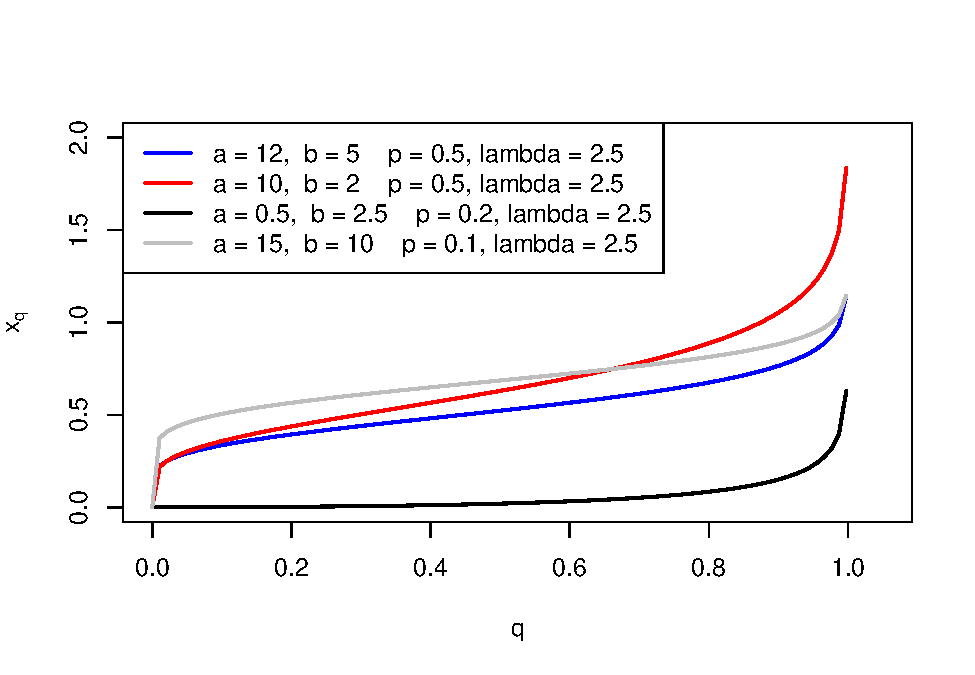
\includegraphics{Kumaraswamy_Marshall-Olkin_Exponential_distribution_files/figure-latex/unnamed-chunk-1-1.pdf}

\begin{Shaded}
\begin{Highlighting}[]
\NormalTok{rKwMOE }\OtherTok{\textless{}{-}} \ControlFlowTok{function}\NormalTok{(n, a, b, p, lambda)}
\NormalTok{\{}
\NormalTok{    U }\OtherTok{\textless{}{-}} \FunctionTok{runif}\NormalTok{(n)}
\NormalTok{    x\_q }\OtherTok{\textless{}{-}}\NormalTok{ (}\DecValTok{1}\SpecialCharTok{/}\NormalTok{lambda)}\SpecialCharTok{*}\FunctionTok{log}\NormalTok{( (}\DecValTok{1} \SpecialCharTok{{-}}\NormalTok{ p}\SpecialCharTok{*}\NormalTok{(}\DecValTok{1}\SpecialCharTok{{-}}\NormalTok{(}\DecValTok{1}\SpecialCharTok{{-}}\NormalTok{U)}\SpecialCharTok{\^{}}\NormalTok{(}\DecValTok{1}\SpecialCharTok{/}\NormalTok{b))}\SpecialCharTok{\^{}}\NormalTok{(}\DecValTok{1}\SpecialCharTok{/}\NormalTok{a) ) }\SpecialCharTok{/}\NormalTok{ (}\DecValTok{1} \SpecialCharTok{{-}}\NormalTok{ (}\DecValTok{1}\SpecialCharTok{{-}}\NormalTok{(}\DecValTok{1}\SpecialCharTok{{-}}\NormalTok{U)}\SpecialCharTok{\^{}}\NormalTok{(}\DecValTok{1}\SpecialCharTok{/}\NormalTok{b))}\SpecialCharTok{\^{}}\NormalTok{(}\DecValTok{1}\SpecialCharTok{/}\NormalTok{a)) )}
\NormalTok{    x\_q}
\NormalTok{\}}

\NormalTok{params }\OtherTok{\textless{}{-}} \FunctionTok{list}\NormalTok{(}\AttributeTok{a=}\FunctionTok{c}\NormalTok{(}\FloatTok{12.0}\NormalTok{,}\FloatTok{10.0}\NormalTok{,}\FloatTok{0.5}\NormalTok{,}\FloatTok{15.0}\NormalTok{),}
               \AttributeTok{b=}\FunctionTok{c}\NormalTok{(}\FloatTok{5.0}\NormalTok{,}\FloatTok{2.0}\NormalTok{,}\FloatTok{2.5}\NormalTok{,}\FloatTok{10.0}\NormalTok{),}
               \AttributeTok{p=}\FunctionTok{c}\NormalTok{(}\FloatTok{0.5}\NormalTok{,}\FloatTok{0.5}\NormalTok{,}\FloatTok{0.2}\NormalTok{,}\FloatTok{0.1}\NormalTok{),}
               \AttributeTok{lambda=}\FunctionTok{c}\NormalTok{(}\FloatTok{2.5}\NormalTok{,}\FloatTok{2.5}\NormalTok{,}\FloatTok{2.5}\NormalTok{,}\FloatTok{2.5}\NormalTok{))}

\FunctionTok{rKwMOE}\NormalTok{(}\AttributeTok{n=}\DecValTok{10}\NormalTok{,}\AttributeTok{a =}\NormalTok{ params}\SpecialCharTok{$}\NormalTok{a[}\DecValTok{1}\NormalTok{],  }\AttributeTok{b =}\NormalTok{ params}\SpecialCharTok{$}\NormalTok{b[}\DecValTok{1}\NormalTok{], }\AttributeTok{p =}\NormalTok{ params}\SpecialCharTok{$}\NormalTok{p[}\DecValTok{1}\NormalTok{], }\AttributeTok{lambda =}\NormalTok{ params}\SpecialCharTok{$}\NormalTok{lambda[}\DecValTok{1}\NormalTok{])}
\end{Highlighting}
\end{Shaded}

\begin{verbatim}
##  [1] 0.2251478 0.5703248 0.5215132 0.6887865 0.3878635 0.4914752 0.5417415
##  [8] 1.0374144 0.4931869 0.5704314
\end{verbatim}

\begin{Shaded}
\begin{Highlighting}[]
\FunctionTok{rKwMOE}\NormalTok{(}\AttributeTok{n=}\DecValTok{10}\NormalTok{,}\AttributeTok{a =}\NormalTok{ params}\SpecialCharTok{$}\NormalTok{a[}\DecValTok{2}\NormalTok{],  }\AttributeTok{b =}\NormalTok{ params}\SpecialCharTok{$}\NormalTok{b[}\DecValTok{2}\NormalTok{], }\AttributeTok{p =}\NormalTok{ params}\SpecialCharTok{$}\NormalTok{p[}\DecValTok{2}\NormalTok{], }\AttributeTok{lambda =}\NormalTok{ params}\SpecialCharTok{$}\NormalTok{lambda[}\DecValTok{2}\NormalTok{])}
\end{Highlighting}
\end{Shaded}

\begin{verbatim}
##  [1] 0.5526452 0.2787452 1.2713657 0.5274659 1.0018385 0.9672524 0.9655029
##  [8] 0.8179552 1.0150983 0.5826127
\end{verbatim}

\begin{Shaded}
\begin{Highlighting}[]
\FunctionTok{rKwMOE}\NormalTok{(}\AttributeTok{n=}\DecValTok{10}\NormalTok{,}\AttributeTok{a =}\NormalTok{ params}\SpecialCharTok{$}\NormalTok{a[}\DecValTok{3}\NormalTok{],  }\AttributeTok{b =}\NormalTok{ params}\SpecialCharTok{$}\NormalTok{b[}\DecValTok{3}\NormalTok{], }\AttributeTok{p =}\NormalTok{ params}\SpecialCharTok{$}\NormalTok{p[}\DecValTok{3}\NormalTok{], }\AttributeTok{lambda =}\NormalTok{ params}\SpecialCharTok{$}\NormalTok{lambda[}\DecValTok{3}\NormalTok{])}
\end{Highlighting}
\end{Shaded}

\begin{verbatim}
##  [1] 8.449836e-05 1.618830e-01 6.516792e-02 5.175740e-02 9.727499e-02
##  [6] 4.657831e-02 3.764357e-02 2.807418e-03 1.341203e-02 4.316365e-02
\end{verbatim}

\begin{Shaded}
\begin{Highlighting}[]
\FunctionTok{rKwMOE}\NormalTok{(}\AttributeTok{n=}\DecValTok{10}\NormalTok{,}\AttributeTok{a =}\NormalTok{ params}\SpecialCharTok{$}\NormalTok{a[}\DecValTok{4}\NormalTok{],  }\AttributeTok{b =}\NormalTok{ params}\SpecialCharTok{$}\NormalTok{b[}\DecValTok{4}\NormalTok{], }\AttributeTok{p =}\NormalTok{ params}\SpecialCharTok{$}\NormalTok{p[}\DecValTok{4}\NormalTok{], }\AttributeTok{lambda =}\NormalTok{ params}\SpecialCharTok{$}\NormalTok{lambda[}\DecValTok{4}\NormalTok{])}
\end{Highlighting}
\end{Shaded}

\begin{verbatim}
##  [1] 0.8336210 0.5622846 0.9744985 0.5206763 0.9443790 0.7148333 0.8983664
##  [8] 1.0717769 0.7734558 0.6627922
\end{verbatim}

\begin{Shaded}
\begin{Highlighting}[]
\NormalTok{x }\OtherTok{\textless{}{-}} \FunctionTok{rKwMOE}\NormalTok{(}
        \AttributeTok{n =} \DecValTok{10000}\NormalTok{,}
        \AttributeTok{a =}\NormalTok{ params}\SpecialCharTok{$}\NormalTok{a[}\DecValTok{1}\NormalTok{],}
        \AttributeTok{b =}\NormalTok{ params}\SpecialCharTok{$}\NormalTok{b[}\DecValTok{1}\NormalTok{],}
        \AttributeTok{p =}\NormalTok{ params}\SpecialCharTok{$}\NormalTok{p[}\DecValTok{1}\NormalTok{],}
        \AttributeTok{lambda =}\NormalTok{ params}\SpecialCharTok{$}\NormalTok{lambda[}\DecValTok{1}\NormalTok{]}
\NormalTok{    )}
\FunctionTok{hist}\NormalTok{(x, }\AttributeTok{prob =}\NormalTok{ T)}
\NormalTok{y }\OtherTok{\textless{}{-}} \FunctionTok{seq}\NormalTok{(}\FloatTok{0.1}\NormalTok{, }\DecValTok{100}\NormalTok{, }\FloatTok{0.0001}\NormalTok{)}
\FunctionTok{lines}\NormalTok{(}
\NormalTok{    y,}
    \FunctionTok{dKwMOE}\NormalTok{(}
\NormalTok{        y,}
        \AttributeTok{a =}\NormalTok{ params}\SpecialCharTok{$}\NormalTok{a[}\DecValTok{1}\NormalTok{],}
        \AttributeTok{b =}\NormalTok{ params}\SpecialCharTok{$}\NormalTok{b[}\DecValTok{1}\NormalTok{],}
        \AttributeTok{p =}\NormalTok{ params}\SpecialCharTok{$}\NormalTok{p[}\DecValTok{1}\NormalTok{],}
        \AttributeTok{lambda =}\NormalTok{ params}\SpecialCharTok{$}\NormalTok{lambda[}\DecValTok{1}\NormalTok{]}
\NormalTok{    ),}
    \AttributeTok{lwd =} \DecValTok{2}\NormalTok{,}
    \AttributeTok{col =} \StringTok{"red"}
\NormalTok{)}
\end{Highlighting}
\end{Shaded}

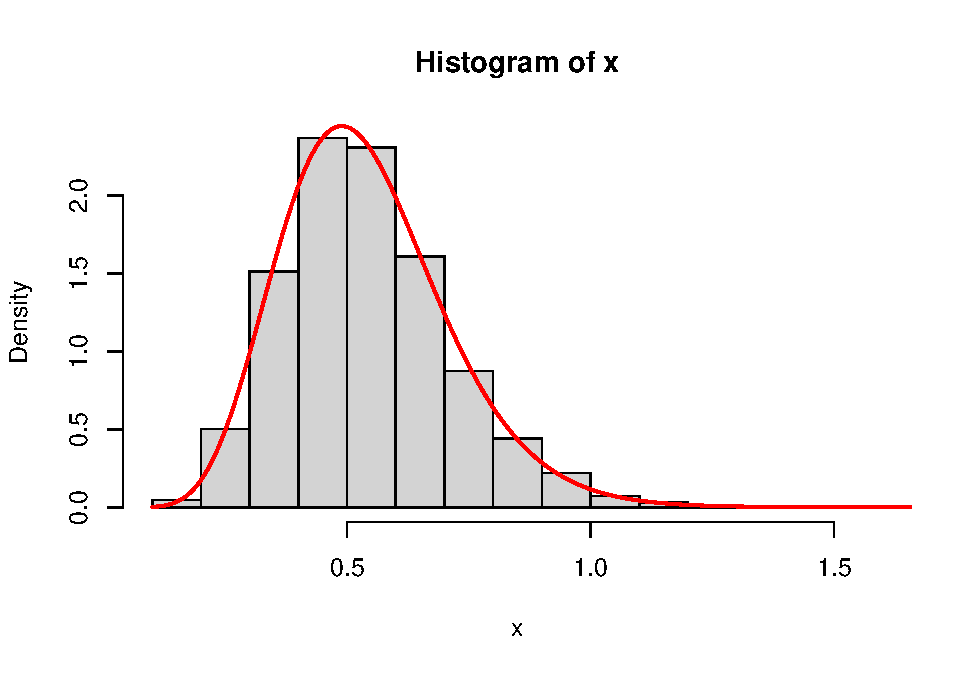
\includegraphics{Kumaraswamy_Marshall-Olkin_Exponential_distribution_files/figure-latex/unnamed-chunk-2-1.pdf}

\hypertarget{fazer-figuras}{%
\section{fazer figuras}\label{fazer-figuras}}

\end{document}
